\documentclass[%
		%draft,
    %submission,
    %compressed,
    final,
    %
    %technote,
    %internal,
    %submitted,
    %inpress,
    reprint,
    %
    %titlepage,
    notitlepage,
    %anonymous,
    narroweqnarray,
    inline,
    twoside,
    invited
    ]{ieee}

\usepackage[utf8]{inputenc}
\usepackage[spanish]{babel}
\usepackage{graphicx}
\usepackage{verbatim}
\usepackage{moreverb}
\usepackage{amsmath}
\usepackage{amsfonts}
\usepackage{amssymb}
\usepackage{fancybox}
\usepackage{float}
\usepackage{fancyvrb}
\usepackage{subfigure}

\newcommand{\latexiie}{\LaTeX2{\Large$_\varepsilon$}}

%\usepackage{ieeetsp}    % if you want the "trans. sig. pro." style
%\usepackage{ieeetc}    % if you want the "trans. comp." style
%\usepackage{ieeeimtc}    % if you want the IMTC conference style

% Use the `endfloat' package to move figures and tables to the end
% of the paper. Useful for `submission' mode.
%\usepackage {endfloat}

% Use the `times' package to use Helvetica and Times-Roman fonts
% instead of the standard Computer Modern fonts. Useful for the 
% IEEE Computer Society transactions.
%\usepackage{times}
% (Note: If you have the commercial package `mathtime,' (from 
% y&y (http://www.yandy.com), it is much better, but the `times' 
% package works too). So, if you have it...
%\usepackage {mathtime}

% for any plug-in code... insert it here. For example, the CDC style...
%\usepackage{ieeecdc}

\begin{document}

%----------------------------------------------------------------------
% Title Information, Abstract and Keywords
%----------------------------------------------------------------------
\title[Redes Neuronales]{%
       Redes Neuronales}

% format author this way for journal articles.
% MAKE SURE THERE ARE NO SPACES BEFORE A \member OR \authorinfo
% COMMAND (this also means `don't break the line before these
% commands).
\author[Castiglione, Karpovsky, Sturla]{Gonzalo V. Castiglione, Alan E. Karpovsky, Martín Sturla\\\textit{Estudiantes 
       Instituto Tecnológico de Buenos Aires (ITBA)}\\
\textbf{3 de Mayo de 2012}
}


\journal{Cátedra\ \ Sist.\ de\ Inteligencia\ Artificial,\ ITBA\ }
\titletext{-\ 3, MAYO\ 2012}
\ieeecopyright{\copyright\ 2012 ITBA}
\lognumber{}
\pubitemident{}
\loginfo{3 de Mayo, 2012.}
\firstpage{1}

\confplacedate{Buenos Aires, Argentina, 3 de Mayo, 2012}

\maketitle               

\begin{abstract} 
El presente informe busca analizar redes neuronales multicapa utilizando funciones de activacion exponencial y tangente hiperbólica, 
para la resolucion del problema dado.

\end{abstract}

\begin{keywords}
Perceptrón, función de transferencia, red neuronal, aprendizaje supervisado, conjunto de entrenamiento, conjunto de testeo
\end{keywords}

%----------------------------------------------------------------------
% SECTION I: Introduccion%----------------------------------------------------------------------
\section{Introducción}

\par Se analizó el comportamiento de distintas redes neuronales multicapa para el problema de la generalización 
de una función matemática a partir de un conjunto de datos (puntos de la función).\\
Con este fin se implementó un algoritmo que permite definir la arquitectura y las propiedades de la red neuronal 
a generar de manera de hacer más simple y práctico su estudio. \\


%----------------------------------------------------------------------
% SECTION II: Marco Teórico
%----------------------------------------------------------------------

\section{Desarrollo}

\subsection{Modelado del problema}

\par Se representó la red neuronal como una \textbf{matriz de pesos}. Cada neurona es una columna de pesos, cada capa de 
neuronas es una matriz de pesos, la red neuronal, por consiguiente, es un vector de matrices. Lo interesante es que hallar 
la salida de la red neuronal con una cierta entrada se reduce a multiplicar el vector entrada por cada una de estas matrices. Cabe destacar 
que al vector y a todos los pasos intermedios se les agrega siempre un $-1$ como último valor para el sesgo.\\
Además de la matriz de pesos se mantiene una matriz paralela representando bajas lógicas a la matriz de pesos. 
Esto permite modelar también redes neuronales no completas ( es decir, no todas las neuronas de una capa 
están conectadas con todas las de la anterior).

\subsection{Elección de puntos}
\par Se optó por escribir funciones que permitan tomar subconjuntos de forma aleatoria del conjunto 
de muestras de entrada, dado un determinado porcentaje. Esto es verdaderamente útil 
si se quiere probar el poder de generalización de la red: Se toma, por ejemplo, un 
conjunto de entrenamiento con el $30\%$ de los valores de entrada y el $70\%$ restante de los puntos 
se asignan al conjunto de testeo (siempre se toman disjuntos). \\
Se decidió tomar una muestra al azar dado que es más leal a situaciones reales en las cuales 
uno debe entrenar la red con los puntos que posee, y no con los que desea. Uno podría, por ejemplo, 
estimar las derivadas parciales de los puntos dados, y utilizar como muestra más representativa 
un conjunto de puntos en los cuales se toma más puntos en donde la norma del gradiente sea mayor, sin embargo 
se decidió no hacerlo por lo ya mencionado.

\subsection{Función de costo}

Como función de costo se decidió implementar únicamente la diferencia cuadrática.


\subsection{Funciones de activación}

\par Para todos los casos de prueba se entrenó a la red utilizando la función de activación la función tangente hiperbólica

\begin{equation}
f(x) = tanh(\beta x)
\end{equation}


y la función exponencial

\begin{equation}
g(x) = \frac{1}{1+e^{-2 \beta x}}
\end{equation}

El programa permite elegir entre ambas para las pruebas. Sin embargo se prefirió utilizar la tangente hiperbólica, dado que :
\begin{equation}
g(x) = \frac{f(x) + 1}{2}
\end{equation}
En otras palabras el comportamiento de las funciones es muy similar, simplemente su imagen es distinta. Nótese que las 
expresiones de los cambios en los pesos de las neuronas tienen como factor el valor  obtenido 
por la función de activación. Dado que la función exponencial satura en $0$ para valores negativos grandes, se 
hace que sea muy difícil cambiar los pesos una vez que comienza la saturación.

\subsection{Normalización de datos}

\par En este problema en particular, los valores de las muestras de entrada $f(x,y) = z$ tenían las siguientes características: Aproximadamente $x\in [-3,3]$, $y\in [-3,3]$ y $z\in [0,1]$. 
Como se comentó anteriormente, la red neuronal puede funcionar con la función de activación tangente hiperbólica 
en todas sus capas o con la función exponencial. En el caso de optar por utilizar la primera de ellas, la imagen de la 
función tangente hiperbólica es $(-1,1)$ y debido a esto se debieron normalizar los valores de $x$ e $y$ y llevarlos 
al $(-1,1)$. Para hacer esto se dividió al vector  $\vec{x}$ por el máximo número en valor absoluto y se realizó el 
procedimiento análogo para el vector $\vec{y}$ ($\vec{x}$ contiene todos los puntos $x$ de las muestras 
de entrada e $\vec{y}$ los puntos $y$).\\
\par Asimismo, teniendo en cuenta que $z$ toma valores entre $0$ y $1$, se decidió utilizar la función de activación 
exponencial en la capa de salida. Como cada capa es independiente de las demás, pueden utilizarse distintas 
funciones de activación en cada capa (lógicamente utilizando la misma función para todas las neuronas de una misma capa). 
Realizando esta pequeña modificación subsanamos el problema de comparar valores que están entre $(-1,1)$ 
(salida de la red neuronal con función de activación tangente hiperbólica en la última capa) con valores de $z$ que están entre $(0,1)$.

\subsection{Procesamiento por lotes}

\par Se decidió procesar las entradas por lotes. Esto significa que una vez mezclados los patrones de entrada, en cada época, 
se procesan $n$ patrones, se calculan los cambios en pesos que se debe hacer para cada uno, y una vez terminado el lote, 
se aplican todos los cambios. Lotes más grandes implican menores costos de procesamiento, pero también implica un 
mayor riesgo de que se cancelen los cambios en los pesos y no se aprenda nada.

\subsection{Mejoras}

\subsubsection{Tasa de aprendizaje}

\par Se implementaron tres tipos de funciones para modificar la variable $\eta$ \textit{(learn rate)}: 
La primera de ellas es a valor \textbf{constante}. La segunda es \textbf{\textit{annealed}} que reduce $\eta$ exponencialmente.
Por último se tiene un \textit{learning rate} \textbf{adaptative} que modifica $\eta$ en función de los últimos errores obtenidos. 
El crecimiento es aritmético, con cota en $\eta =0.5$, la reducción es exponencial. La idea de dicha regla es la siguiente: 
si el error se disminuye consistentemente, es posbile que la tasa sea demasiado chica, ya que se está siendo muy conservador 
y se podría disminuir el error a mayor velocidad. Si el error incrementa, la tasa es demasiado grande, por lo cual se reduce.\\

\subsubsection{Cambios con momento}

\par Se decidió implementar que los cambios de pesos de la red sean con momento. Esto significa que los cambios de los 
pesos está dado por:
\[w_{ij}(t+1)= - \frac{\partial E}{\partial w{ij}} + \alpha w(t)\]
Lo cual significa que al cambio normal (primer término) se le suma una parte de los cambios anterior. Esto hace 
que los cambios tomen una cierta inercia y pesen aún en los próximos cambios. Nótese que hay un olvido exponencial 
de los cambios anteriores.
\subsubsection{Escape de mínimos locales}

\par En iteraciones anteriores, debido a la existencia de mínimos locales se desarrolló un algoritmo  
\textbf{\textit{persistent search}} que intentaba 
escapar de dichos mínimos utilizando reinicios luego de cierta cantidad de épocas ( se tiran los pesos, se toman otros).
\par Se decidió descartar dicho algoritmo en favor de agregar ruido a los pesos de la red. Debido a la robustez de 
las redes neuronales, a largo plazo dicho peso no debería tener un impacto en el error. Por otra parte, dicho 
ruido podría ser lo necesario para que la red escape de un mínimo local. Teniendo en cuenta ambas cosas, se decidió
agregar ruido estocásticamente al finalizar el procesamiento de cada lote. Al finalizar cada lote, con una cierta probabilidad, 
para cada capa de conexiones, se elije una conexión al azar y se le agrega un ruido proporcional a su valor.

\subsection{Arquitecturas}

\par  La elección de arquitecturas es crucial para el aprendizaje de la red. Las arquitecturas inadecuadas podrían quizás no 
alcanzar una cierta cota de error en el conjunto de entrenamiento, incluso para una cantidad arbitrarias de épocas. Otras 
arquitecturas podrían, por ejemplo, memorizar bien ( reducir el error en el conjunto de entrenamiento) pero generalizar 
mal ( reducir el error en el conjunto de testeo).

\subsubsection{Arquitecturas sin capa oculta}

También denominadas perceptres simples, dichas arquitecturas están atadas a la naturaleza de los conjuntos de entrada 
y salida. En el caso particular de dos entradas y una salida, la red se reduce a computar:
\begin{equation}
O(x,y) = tanh(\beta (ax+by - k))
\end{equation}
La red intentará hallar valores $a,b,k$ ( siendo $a,b$ pesos de conexiones, $k$ el sesgo) 
tal que la función de costo esté minimizada en los puntos dados. Si la función 
tiene un comportamiento muy distinto al de la función de activación, poco podrán reducir el error dichas redes. 
Debido a esta gran limitación, se decidió no usar perceptrones simples.

\subsubsection{Arquitecturas con pocas neuronas y capas}

\par Estas redes sufren un problema similar al de los perceptrones simples. Debido a la baja cantidad de neuronas 
en comparación con la complejidad de la función, es posible que incluso en una cantidad arbitraria de épocas 
el error pueda no disminuir por debajo de ciertos valores. En el ejemplo anterior, al tener una expresión muy 
clara de la salida de la red, este fenómeno era más obvio. A pesar de que analíticamente no sea tan trivial en este caso, 
en los gráficos producidos por estas redes se puede apreciar como el error nunca alcanza valores por debajo de 
ciertas cotas. 
\par Sin embargo, debido a las limitaciones ya dichas, estas redes son comparativamente buenas generalizando. Esto 
se puede apreciar gráficamente con curvas del error de entrenamiento y posterior testeo muy similares. 

\par Ejemplos particulares de dichas redes incluyen arquitecturas con, por ejemplo, 4 neuronas en la primer capa oculta y 4
en la segunda ( para el problema en cuestión). Ver \textbf{Anexo a} figura $1$.

\subsubsection{Arquitecturas con muchas neuronas y muchas capas}

\par Estas redes tienen capacidades expresivas mucho mayores que las ya mencionadas anteriormente. Esto hace que se puedan 
alcanzar cotas de errores mucho menores, incluso casi nulas. El problema con dichas redes es que tienden a memorizar. Si 
se intenta reducir el error a valores crecientemente bajos, es posible que los errores en los patrones de testeo comiencen 
a crecer. El fenómeno que ocurre es análogo a querer aproximar ocho puntos sobre una línea recta utilizando un polinomio 
de grado $7$; se puede interpolar perfectamente, el error de los puntos sería $0$, pero al tomar otros puntos sobre 
la línea recta el error sería particularmente alto.

\par Cabe destacar que dichas redes demoran considerablemente más en entrenarse en 
una cierta cantidad de épocas debido 
a la complejidad de efectuar un algoritmo \textit{back-propagation} en redes grandes. 

\subsubsection{Arquitecturas intermedias}

\par En vista de las dos secciones anteriores, existe un compromiso entre la capacidad de reducir el error aribtrariamente 
y la capacidad de generalización. Por lo tanto, se prefirió escoger un punto medio en el cual la generalización sea buena y 
el error sea relativamente bajo ( es decir, la precisión dado un cierto error razonable es alta y similar en tanto 
el conjunto de aprendizaje o entrenamiento y testeo). También se observó que redes más pequeñas son más veloces ( 
no solo en término de tiempo, sino de épocas) en reducir el error.

\par Los fenómenos mencionados pueden ser observados en el \textbf{Anexo A} , figuras $1$ y $2$. El primero 
muestra como el error de entrenamiento y testeo se separan considerablemente de por momentos (peor generalización) y 
por otro lado la tendencia a reducir el error es más lenta.

\subsubsection{Arquitecturas no simétricas}

\par La teoría detrás de las redes neuronales no exige que las redes sean completas ( es decir, que todas 
las neuronas entre dos capas están conectadas todas entre sí). Las redes deberían incluso, debido a su robustez, poder soportar 
que se rompa una conexión durante el entrenamiento y adaptarse. Debido a esto, 
se decidió a manera experimental probar con arquitecturas no simétricas, 
es decir, arquitecturas en las cuales la primer capa no es completa ( existen conexiones muertas), con condiciones razonables ( que la salida sea 
alcanzable desde toda entrada, por ejemplo). 
\par Dicha implementación no generó mejoras consistentes como para preferirla sobre redes simétricas, pero tampoco 
obtuvieron resultados consistentemente peores como para descartarlas por completo.

\section{Cálculo del error}

\par Para los gráficos se optó por mostrar la \textbf{diferencia cuadrática media} calculada como sigue:\\

\begin{equation}
\sum\limits_{i}\frac{(S_i - O_i)^{2}}{N}
\end{equation}

\par En cuanto al error, se calcula el \textbf{error promedio} de la siguiente forma:

\begin{equation}
e = \sum\limits_{i}\frac{|S_i - O_i|}{N}
\end{equation}


Entonces, esto está diciendo, por ejemplo que, si la sumatoria es igual a 0.01, cada valor tiene un error promedio de 0.01.

\par Por ultimo se calculó la \textbf{desviación del valor absoluto error}:\\

\begin{equation}
\sqrt{\sum\limits_{i}\frac{((\|S_i - O_i\| - e))^2}{N}}
\end{equation}

Si, por ejemplo, el desvío es igual a 0, significaría que todos los valores tienen un error de
0.01. Es decir el error es fijo. Si es alto significa que hay algunos valores muy precisos (error casi 0) y otros con errores grandes. Es decir el error es variado.

\section{Resultados}

\par En las pruebas realizadas con el factor de momentum activado se observó que la red no se estanca tan fácilmente en mínimos locales. Sin embargo, en algunos casos, puede demorar la convergencia de la red hacia los valores deseados, 
debido a la memorización de cambios quizás no deseados.\\

\par Las arquitecturas con una cantidad moderada de neuronas en dos capas fueron las que dieron los 
mejores resultados. 
Con una arquitectura con $50$ neuronas en la primer capa oculta y $30$ en la segunda, se logró alcanzar un error medio de 
$0.046$ y desviación de $0.018$ en tan solo 200 épocas. Esto se tradujo a un coeficiente superior a $0.8$ tanto para el conjunto de entrenamiento 
y el de testeo para un error de $0.05$.

\par Asimismo se observó que la función de activación tangente hiperbólica resultó obtener una mejor performance en comparación con la función sigmoidea exponencial.

\par Por su parte es notoria la diferencia en cantidad de épocas de la red funcionando con un $\eta$ adaptativo versus la red funcionando sin este. Mejor aún, la reducción en el número de épocas utilizando $\eta$ adaptativo es superior al $25\%$.\\

\par De todas formas, los resultados obtenidos no pueden ser descartados y/o tomados como óptimos o 
absulutos. Esto se debe a que el problema presenta numerosas variables 
que pueden incidir en el resultado del aprendizaje de una red neuronal: 
los distintos valores que pueden tomar $\beta$ y $\eta$, la arquitectura utilizada, 
la cantidad de épocas, la presencia de ruido aleatorio, las conexiones muertas para romper simetría, etc.\\

\par Además, debido a la aleatoriedad de la elección de los puntos a utilizar en el conjunto de entrenamiento y la inicialización de los pesos de a red al azar, no podemos dar por descartadas malos resultados ya que es posible que, por ejemplo, se hayan seleccionado puntos poco representativos de la función o que los pesos no se hayan inicializado de la forma óptima.
\par Una forma de subsanar esta problemática sería correr numerosas veces cada caso de testeo antes de poder sacar una conclusión con la tendencia, pero debido a la complejidad temporal del problema ( sobre 
todo para redes grandes) , realizar esto requeriría más tiempo que el disponible.

\section{Conclusión}

Luego de realizadas las pruebas y analizado los resultados, se pudo observar lo siguiente:\\
\begin{itemize}
\item Incrementar la cantidad de neuronas arbitrariamente no necesariamente 
implica mejoras en cuanto al error (puede llevar a malas generalizaciones y tiempo de más 
hasta alcanzar el error desdeado). Esto puede observarse en la figura 1 del \textbf{Anexo A}\\
\item No existe tal cosa como una mejor arquitectura o parámetros óptimos. Estos seguramente dependan 
el problema que se está analizando.\\
\item Momentum no siempre puede acelerar la convergencia.\\
\item La función de activación \textit{exponencial} es más propensa a atascarse en mínimos.
\item Tomar pocos puntos puede ser una muestra poco representativa, y por lo tanto, puede haber 
mala generalización.\\
\end{itemize}


%----------------------------------------------------------------------


\clearpage
\onecolumn

\section*{Anexo A: Gráficos}

\begin{figure}[H]
\begin{center}
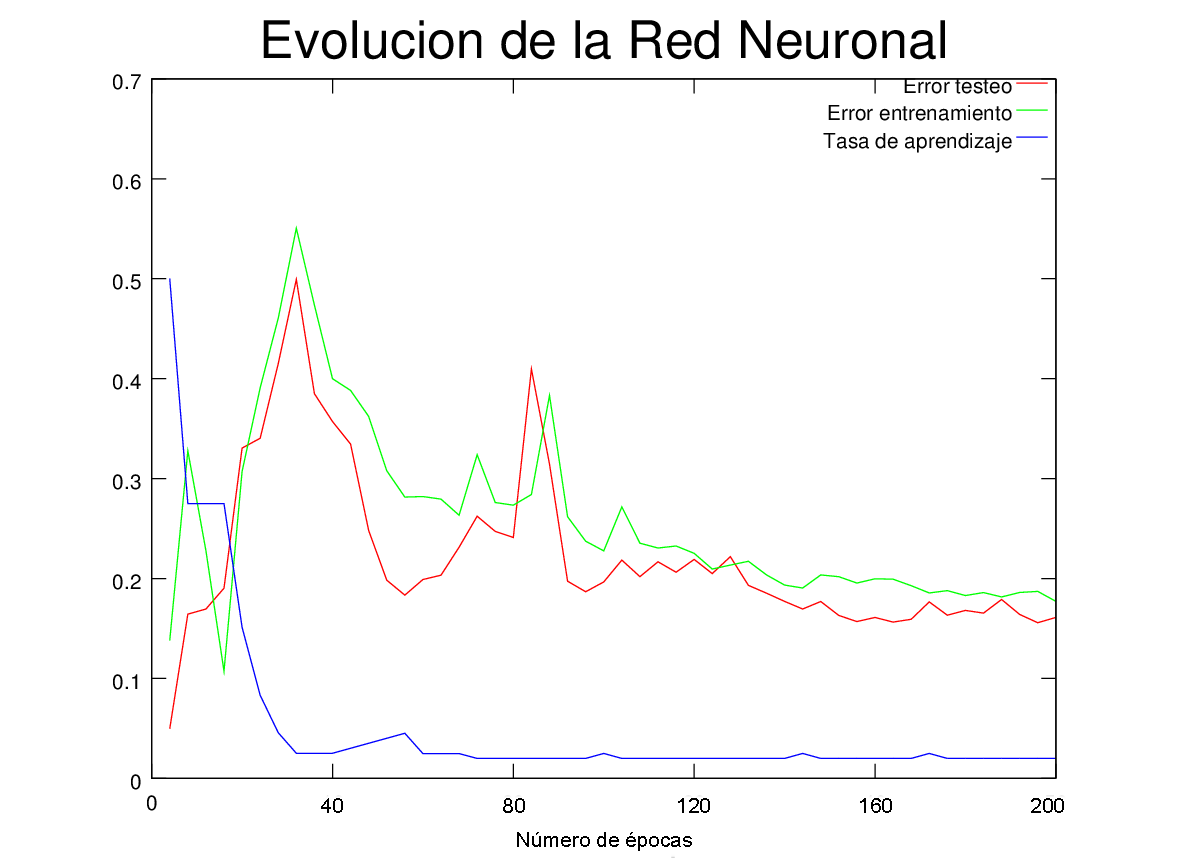
\includegraphics[scale=0.70]{./images/6.png}
\label{modelado}
\end{center}
\end{figure}

\begin{center}
\par Figura 1: Ejemplo red neuronal con una arquitectura de [200 100] entrenada 200 épocas con learning rate adaptativo y función de activación tangente hiperbólica.  
La tendencia muestra que el error baja, pero lentamente.
\end{center}

\begin{figure}[H]
\begin{center}
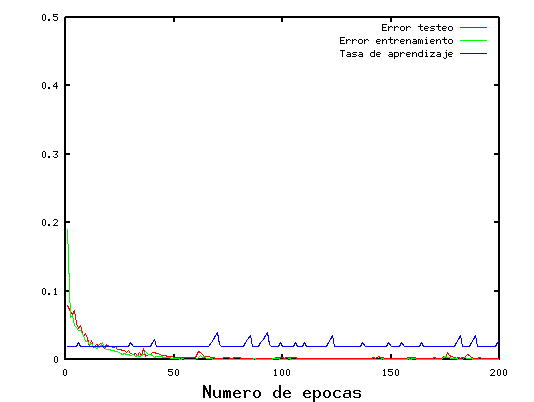
\includegraphics[scale=0.70]{./images/nice.png}
\label{modelado}
\end{center}
\end{figure}

\begin{center}
\par Figura 2: Ejemplo red neuronal con una arquitectura de [50 30] entrenada 200 épocas con learning rate adaptativo y función de activación tangente hiperbólica. 
Se alcanzó un error medio de aproximadamente 0.05 y desviación 0.018.
\end{center}
\clearpage

\begin{figure}[H]
\begin{center}
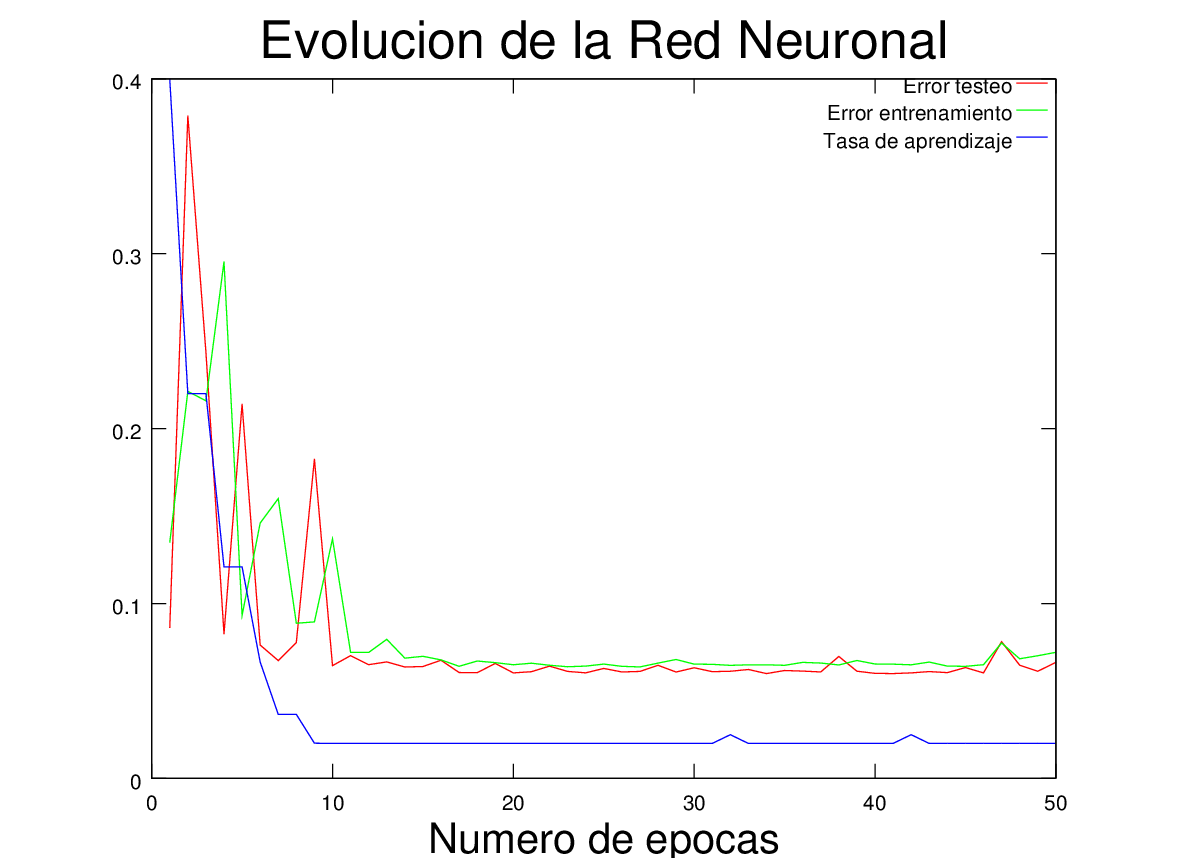
\includegraphics[scale=0.70]{./images/9.png}
\label{modelado}
\end{center}
\end{figure}

\begin{center}
\par Figura 3: Ejemplo red neuronal con una arquitectura de [4 4] entrenada 200 épocas con learning rate adaptativo y función de activación tangente hiperbólica. 
El error no baja de más de 0.08 sin importar cuántas épocas itere.
\end{center}




%\VerbatimInput{./code/calculoAb.m}




\end{document}